La introducción de sistemas de TI complejos requiere de un enfoque estructurado de gestión de todos los pasos que hay en el ciclo de vida del proyecto desde su concepción hasta su puesta en práctica y mejora continua. En el presente trabajo se utilizó la metodología PPDDIO (Prepare, Plan, Design, Develop, Implement, Operate, Optimize) ajustada a las características concretas de una solución basada en blockchain para gestionar y comprobar registros de seguridad. Este capítulo explica para cada paso cómo se desarrolló la aplicación práctica de esta metodología y cómo se utilizó esta metodología para asegurar una evolución ordenada, eficaz y segura en el desarrollo del sistema.


\subsection{Fase 1: Preparación}
En esta etapa del trabajo se examinaron los principales métodos tradicionales utilizados para almacenar y gestionar logs de seguridad en sistemas informáticos. El análisis permitió identificar deficiencias estructurales que comprometen la confiabilidad de los registros, especialmente en escenarios donde se requiere integridad, trazabilidad y autenticidad para fines de auditoría y análisis forense. Métodos como el almacenamiento en archivos planos, bases de datos relacionales, syslog tradicional o el uso de discos locales presentan vulnerabilidades que pueden ser explotadas sin dejar evidencia detectable.

La Tabla~\ref{tab:analisis-logs} resume los hallazgos de esta evaluación, destacando las limitaciones específicas de cada método en relación con los principios de seguridad. Se evidencia que ninguno de estos enfoques ofrece garantías sólidas frente a la manipulación o falsificación de registros, lo que justifica la necesidad de explorar alternativas más robustas como el uso de tecnología blockchain.
\\
\\
\\
\\
\\
\\
\\

\begin{table}[ht]
\centering
\captionsetup{list=no}
\caption{ANÁLISIS DE MÉTODOS TRADICIONALES DE ALMACENAMIENTO Y GESTIÓN DE LOGS DE SEGURIDAD}
\addcontentsline{lot}{table}{Tabla \thetable. Análisis de métodos tradicionales de almacenamiento y gestión de logs de seguridad}
\begin{tabularx}{\textwidth}{>{\raggedright\arraybackslash}X 
                                    >{\raggedright\arraybackslash}X 
                                    >{\raggedright\arraybackslash}X 
                                    >{\raggedright\arraybackslash}X 
                                    >{\raggedright\arraybackslash}X}
\toprule
\textbf{Método Tradicional} & \textbf{Descripción} & \textbf{Limitaciones en Integridad} & \textbf{Limitaciones en Trazabilidad} & \textbf{Limitaciones en Autenticidad} \\
\midrule
Archivos de texto plano (flat files) & Registros guardados en archivos \textit{.log} o \textit{.txt} locales o en servidores. & Vulnerables a manipulaciones sin dejar rastro \cite{casey2011}. & No permiten verificar de forma confiable la secuencia de eventos \cite{bishop2003}. & No hay validación de origen del log \cite{marty2008}. \\
\addlinespace
Bases de datos relacionales (SQL) & Uso de DBMS como MySQL o PostgreSQL para almacenar registros. & Los registros pueden ser editados sin dejar historial claro \cite{bishop2003}. & Requieren configuraciones avanzadas para asegurar trazabilidad. & Carecen de mecanismos nativos de firma digital \cite{casey2011}. \\
\addlinespace
Syslog tradicional (RFC 3164) & Protocolo de registro estándar en sistemas UNIX. & No incluye mecanismos de verificación de integridad \cite{gerhards2009}. & No garantiza orden exacto ni origen seguro \cite{gerhards2009}. & Los mensajes pueden falsificarse o interceptarse \cite{gerhards2009}. \\
\addlinespace
Correo electrónico de alertas & Envío de logs críticos a correos definidos. & El contenido puede alterarse en tránsito si no se cifra \cite{kent2006}. & No hay secuencia temporal confiable o sincronizada \cite{kent2006}. & Difícil verificar emisor sin firmas digitales \cite{kent2006}. \\
\addlinespace
Almacenamiento en discos locales & Logs almacenados directamente en discos duros locales. & Vulnerables a pérdidas o modificaciones por fallos o accesos \cite{kent2006}. & Difícil relacionar eventos si no hay sincronización horaria \cite{bishop2003}. & Falta de verificación de legitimidad del evento \cite{marty2008}. \\
\bottomrule
\end{tabularx}
\label{tab:analisis-logs}
\end{table}

Con base en este análisis, se estudian tecnologías que pudieran garantizar integridad, trazabilidad y resistencia a la manipulación. Se selecciona la tecnología blockchain, concretamente Hyperledger Fabric, por su arquitectura permisionada, su control de acceso granular y su soporte para smart contracts.

Se determinaron los requerimientos técnicos necesarios, especificando las versiones exactas de cada componente para garantizar la reproducibilidad y compatibilidad del sistema:
\begin{itemize}
\item \textbf{Subsistema de Windows para Linux (WSL2)} con Ubuntu 22.04.5 LTS (Jammy) y kernel Linux 5.15.153.1-microsoft-standard-WSL2 para la organización del ámbito de desarrollo, proporcionando un entorno nativo Linux optimizado.
\item \textbf{Plataforma de contenedorización} mediante Docker 27.5.1 y Docker Compose 1.29.2 para la orquestación de servicios distribuidos de la red blockchain.
\item \textbf{Runtime de desarrollo} con Node.js v22.15.0 y npm 10.9.2 para el desarrollo de aplicaciones cliente y la gestión de dependencias del ecosistema JavaScript.
\item \textbf{Hyperledger Fabric 2.2.15} (Commit SHA: 79c8cc2) como plataforma blockchain permisionada, incluyendo las herramientas nativas peer, configtxgen y cryptogen compiladas con Go 1.21.6.
\item \textbf{Integración con Syslog} mediante protocolo UDP en puerto 5140 para la recogida en tiempo real de logs del sistema operativo, implementando filtrado inteligente de eventos de seguridad.
\item \textbf{Elección de JavaScript} como lenguaje para los smart contracts, aprovechando las capacidades del runtime Node.js v22.15.0 y la compatibilidad nativa con Hyperledger Fabric.
\item \textbf{Infraestructura de seguridad} basada en OpenSSL 3.0.2 para criptografía y certificados TLS, garantizando comunicaciones seguras entre todos los componentes del sistema.
\item \textbf{Herramientas de desarrollo} incluyendo Git 2.34.1 para control de versiones y curl 7.81.0 para pruebas de conectividad y validación de APIs REST.
\item \textbf{Soporte de protocolos} HTTP/HTTPS 1.1/2.0 para interfaces web y APIs, gRPC integrado en Fabric para comunicación blockchain, y UDP para captura de logs Syslog.
\end{itemize}
Dicho conjunto de decisiones posibilitó generar una base técnica consistente con los objetivos del sistema planteado, estableciendo un entorno de desarrollo reproducible que garantiza la compatibilidad entre componentes y facilita tanto el desarrollo iterativo como la eventual transición a entornos de producción.




\subsection{Fase 2: Planificar}
Durante la fase de planificación, se definieron las actividades necesarias para diseñar e implementar un sistema orientado a asegurar los registros de seguridad mediante el uso de tecnología blockchain. Esta etapa tuvo una duración total de cuatro meses y permitió establecer una hoja de ruta clara, así como asignar recursos técnicos y temporales al proyecto.

Inicialmente, se destinaron esfuerzos a la identificación de la tecnología blockchain más adecuada. Tras un análisis comparativo de diferentes alternativas, se optó por \textbf{Hyperledger Fabric}, debido a sus características de código abierto, arquitectura modular y soporte para redes permisionadas, lo cual resulta esencial para entornos corporativos donde la seguridad y el control de acceso son prioritarios.

Posteriormente, se procedió con la revisión detallada de su documentación oficial, el análisis de ejemplos provistos por la comunidad, y la comprensión de su funcionamiento interno, incluyendo la arquitectura de canales, peers, orderers y smart contracts (chaincode).

En paralelo, se exploraron y evaluaron herramientas para la generación y recolección de logs, siendo \textbf{Syslog} una de las candidatas por su compatibilidad con sistemas operativos Unix/Linux y su flexibilidad en la configuración.

Se diseñó la arquitectura de la red de blockchain que se implementaría, definiendo los nodos participantes, los canales de comunicación, las políticas de gobernanza y los puntos de integración con los sistemas de logs. Finalmente, se procedió a la configuración del entorno de desarrollo, utilizando \textbf{WSL (Windows Subsystem for Linux)}, contenedores Docker y dependencias necesarias para la ejecución de Hyperledger Fabric.

La planificación se estructuró conforme a las fases de la metodología PPDIOO, como se muestra en la siguiente tabla:

\begin{table}[H]
\centering
\captionsetup{list=no}
\caption{PLANIFICACIÓN PARA LA IMPLEMENTACIÓN DEL SISTEMA DE ASEGURAMIENTO DE LOGS MEDIANTE BLOCKCHAIN}
\addcontentsline{lot}{table}{Tabla \thetable. Planificación para la implementación del sistema de aseguramiento de logs mediante blockchain}
\label{tabla:planificacion}
\begin{tabular}{|l|c|c|c|c|}
\hline
\textbf{Fase}            & \textbf{Mes 1} & \textbf{Mes 2} & \textbf{Mes 3} & \textbf{Mes 4} \\
\hline
Preparación              & X              &                &                &                \\
\hline
Planificación            & X              &                &                &                \\
\hline
Diseño de red            &                & X              &                &                \\
\hline
Implementación           &                & X              & X              &                \\
\hline
Operación                &                &                & X              &                \\
\hline
Optimización             &                &                &                & X              \\
\hline
\end{tabular}
\end{table}

\subsection{Fase 3: Diseño}
Durante la fase de diseño se definió una arquitectura de red basada en Hyperledger Fabric, orientada a preservar la integridad, trazabilidad y autenticidad de los logs de seguridad generados por los dispositivos. La Fig.~\ref{figura:diseno-red} muestra una versión mínima viable de esta arquitectura, pensada para operar con un único dispositivo, pero con capacidad de escalamiento hacia entornos corporativos de mayor complejidad.
\begin{figure}[H]
\centering
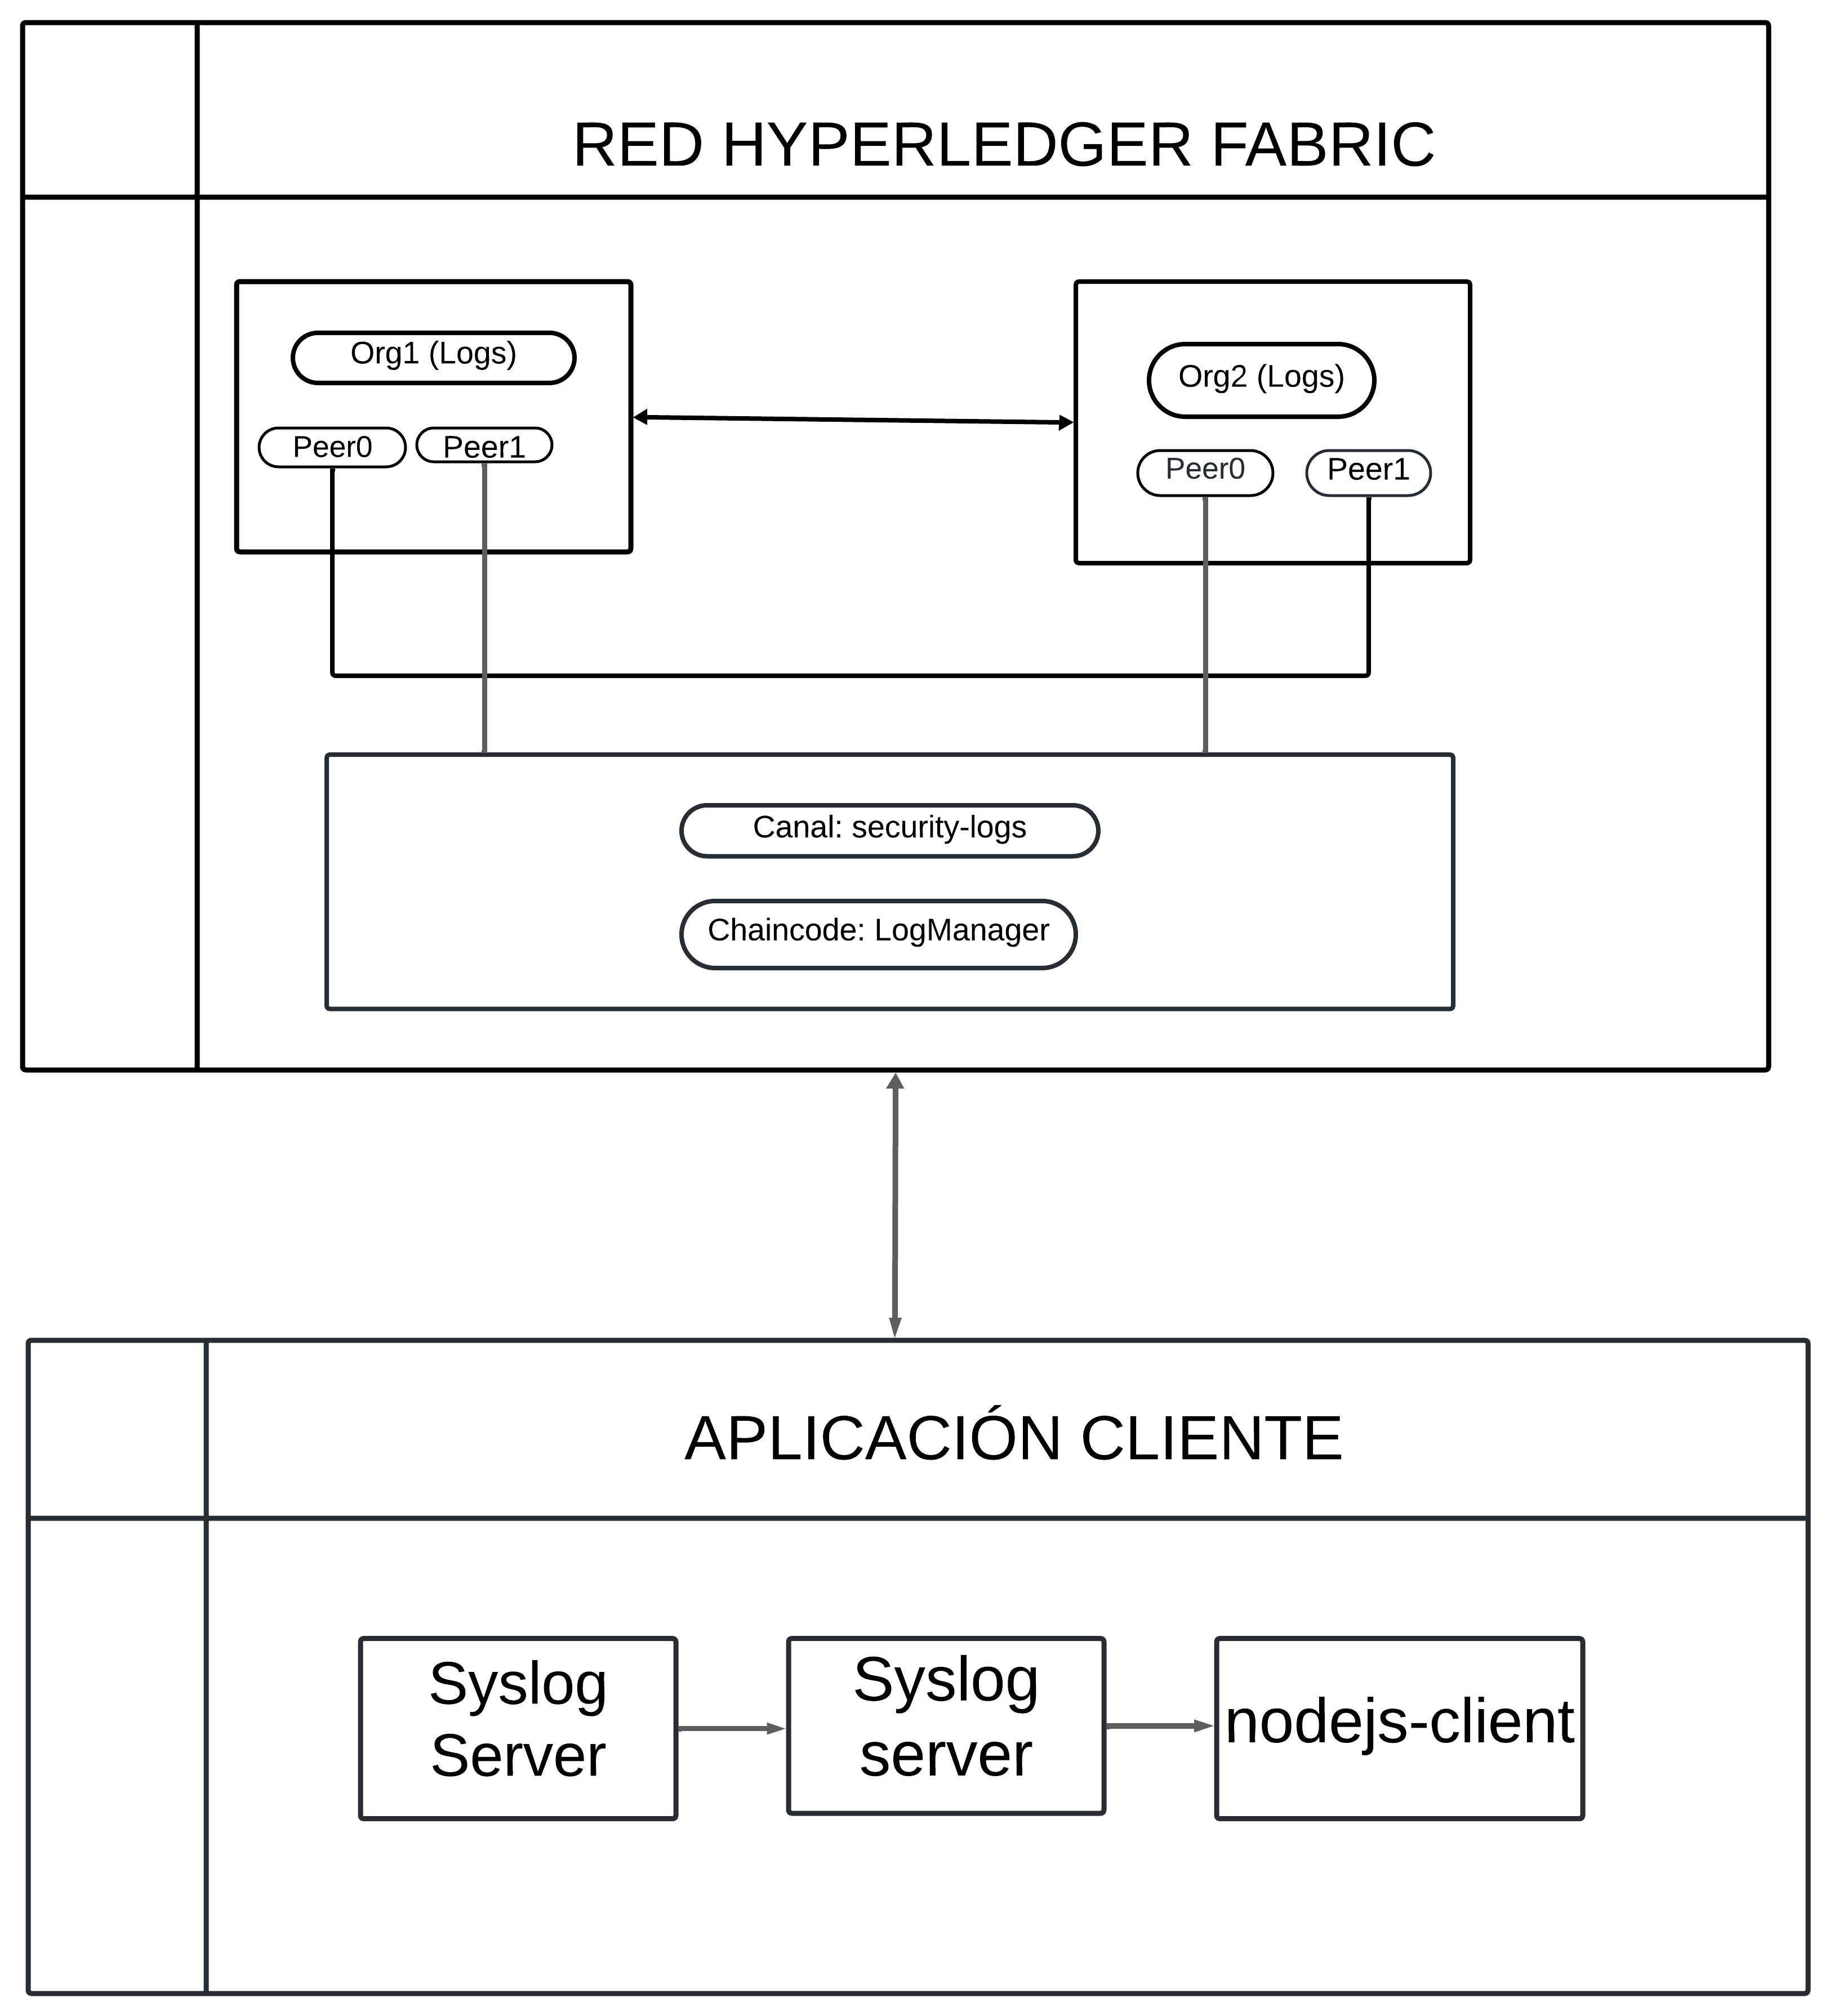
\includegraphics[width=0.70\textwidth]{figuras/Diseno_red_blockchian.png}
\caption{Arquitectura de la red Hyperledger Fabric para gestión de logs de seguridad}
\label{figura:diseno-red}
\end{figure}
La red está conformada por dos organizaciones diferenciadas por sus funciones. La primera, \textit{LogProvider MSP}, se encarga de generar, procesar y enviar los logs a la red blockchain. Representa a la entidad responsable de la administración de los sistemas que producen eventos de seguridad. La segunda, \textit{LogAuditor MSP}, actúa como auditor independiente con la función de validar, verificar y monitorear los registros almacenados, asegurando una capa adicional de control. Esta separación de responsabilidades responde al principio de segregación de funciones, esencial en cualquier sistema de auditoría confiable.


Cada organización cuenta con dos peers identificados como \textit{peer0} y \textit{peer1}, configuración que responde a criterios técnicos específicos orientados a garantizar la disponibilidad y confiabilidad del sistema. El criterio de redundancia asegura que si un nodo experimenta fallos técnicos o se encuentra temporalmente inaccesible, el nodo restante mantiene operativa la red, evitando interrupciones en el servicio de logging.

Desde la perspectiva del consenso, esta configuración cumple con el mínimo requerido para la validación distribuida en redes permisionadas, donde se necesita la participación de múltiples nodos para validar las transacciones. Adicionalmente, el criterio de desempeño permite mejorar el rendimiento en operaciones de consulta mediante balanceo de carga, distribuyendo las peticiones entre los peers disponibles.

La configuración específica de la red incluye puertos dedicados para cada componente, facilitando la administración y el monitoreo del sistema. El \textit{peer0} de LogProvider MSP opera en el puerto 7051 con su base de datos CouchDB correspondiente en el puerto 5984, mientras que el \textit{peer1} funciona en el puerto 8051 con CouchDB en el puerto 6984.
De manera similar, la organización LogAuditor MSP tiene su \textit{peer0} configurado en el puerto 9051 con CouchDB en el puerto 7984, y su \textit{peer1} en el puerto 10051 con CouchDB en el puerto 8984. Esta separación de puertos facilita la escalabilidad del sistema y permite un control granular sobre cada componente de la red.

Se ha configurado un canal denominado \textit{security-logs-channel}, dedicado exclusivamente al intercambio y almacenamiento de registros de seguridad. Este canal proporciona aislamiento y confidencialidad en las operaciones de logging, asegurando que únicamente las organizaciones autorizadas puedan acceder a los datos de seguridad.

El canal actúa como un libro de contabilidad distribuido donde se registran todas las transacciones relacionadas con logs de seguridad, manteniendo un historial inmutable y verificable. Esta aproximación garantiza que los registros no puedan ser alterados una vez confirmados en la blockchain.
Sobre dicho canal se despliega un contrato inteligente denominado security-logs v2.1, el cual contiene la lógica de negocio necesaria para gestionar todo el ciclo de vida de los logs de seguridad. Este \textit{chaincode} implementa funciones especializadas que van más allá del simple almacenamiento de datos.

Las funcionalidades del contrato inteligente incluyen el almacenamiento de registros de logs con codificación Base64 para evitar problemas con caracteres especiales, la ejecución de consultas complejas sobre los registros almacenados utilizando índices optimizados de CouchDB, y la verificación de la integridad de los datos mediante mecanismos de control criptográfico basados en \textit{hashes SHA-256}.
La red blockchain se complementa con una aplicación cliente robusta compuesta por tres módulos interconectados que forman un pipeline completo de procesamiento de logs. Esta arquitectura modular permite una separación clara de responsabilidades y facilita el mantenimiento del sistema.

El primer módulo, implementado en \textit{syslog-collector.js}, actúa como servidor Syslog especializado que recoge logs del sistema operativo a través del puerto UDP 5140. Este componente aplica filtrado inteligente para capturar únicamente eventos críticos de seguridad con severidad igual o menor a WARNING, eventos de autenticación provenientes de SSH, sudo y PAM, errores críticos del kernel y eventos que contengan palabras clave relacionadas con seguridad.
El segundo módulo corresponde al cliente Node.js implementado en \textit{app.js}, que funciona como una \textit{API REST} en el puerto 3000. Este componente procesa los logs recibidos del colector Syslog, los estructura en formato JSON, aplica codificación Base64 para garantizar la integridad durante el transporte, genera firmas criptográficas SHA-256, y los prepara para su envío a la red blockchain mediante invocaciones de chaincode utilizando gRPC sobre TLS.

El tercer módulo consiste en una interfaz web implementada en dashboard.html que proporciona visualización en tiempo real de los logs almacenados en la blockchain. Esta interfaz incluye funcionalidades de auto-actualización cada cinco segundos, decodificación automática de mensajes Base64, filtros avanzados por fuente y severidad, y cálculo de estadísticas en tiempo real como total de logs, logs críticos del día y última actualización.

Este diseño busca lograr un equilibrio óptimo entre simplicidad operacional, seguridad robusta y escalabilidad futura. La arquitectura facilita el desarrollo y la implementación de una prueba de concepto funcional, mientras mantiene la flexibilidad necesaria para evolucionar hacia entornos de producción más complejos.

La solución implementada no compromete las propiedades fundamentales que se desean garantizar en los logs de seguridad: integridad criptográfica mediante hashes inmutables, trazabilidad completa a través del historial blockchain, y autenticidad verificable mediante firmas digitales y control de acceso granular.

\subsection{Fase 4: Implementación}
La fase de implementación representa la transición del diseño conceptual a la construcción práctica del sistema. En este proyecto, se procedió a configurar un entorno de desarrollo controlado donde se desplegó una red de Hyperledger Fabric adaptada para registrar eventos de seguridad provenientes de Syslog. Esta fase incluyó la instalación de herramientas, la creación de scripts de automatización, el desarrollo del smart contracts, la integración de fuentes de datos y la verificación del funcionamiento del sistema en un entorno realista.

Antes de proceder con la implementación, se verificó la compatibilidad entre las versiones de los principales componentes utilizados: Node.js, Docker y Docker Compose. Esta verificación fue fundamental para asegurar la correcta instalación de Hyperledger Fabric y evitar conflictos entre dependencias durante el despliegue de la red.

La Fig.~\ref{figura:versiones-entorno} muestra las versiones empleadas en el entorno de desarrollo. Garantizar esta compatibilidad técnica resultó clave para ejecutar los contenedores de la red, instalar los paquetes necesarios y desplegar el smart contract sin errores de compatibilidad.

\begin{figure}[H]
\centering
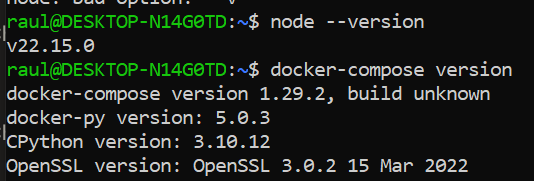
\includegraphics[width=0.70\textwidth]{figuras/instalacion_herramientas.png}
\caption{Versiones de las herramientas de desarrollo}
\label{figura:versiones-entorno}
\end{figure}

\subsubsection{Configuración de la estructura criptográfica}
El primer paso fundamental en la implementación fue la definición de la estructura organizacional y criptográfica de la red mediante el archivo \textit{crypto-config.yaml}. Este archivo especifica la topología de la red blockchain, definiendo las organizaciones participantes, la cantidad de nodos peer por organización y los usuarios autorizados.
La configuración estableció tres entidades principales: OrdererOrg como la organización responsable del servicio de ordenamiento, LogProvider como la organización encargada de generar y enviar los logs de seguridad, y LogAuditor como la entidad auditora con permisos de lectura y validación. Cada organización peer se configuró con dos nodos para garantizar redundancia y alta disponibilidad, mientras que se definió un usuario adicional por organización para operaciones administrativas.
Esta estructura jerárquica permite una separación clara de responsabilidades: la organización OrdererOrg mantiene la neutralidad en el proceso de consenso, LogProvider tiene permisos de escritura para registrar eventos de seguridad, y LogAuditor posee capacidades de auditoría y verificación sin comprometer la integridad del sistema.

\subsubsection{Definición de políticas y perfiles de red}
La configuración de la red se completó mediante el archivo \textit{configtx.yaml}, que define las políticas de gobernanza, las capacidades de la red y los perfiles de configuración necesarios para el despliegue. Este archivo constituye el núcleo de la configuración de Hyperledger Fabric, especificando cómo interactúan las organizaciones y qué operaciones están permitidas.
Se implementó una configuración compatible con Fabric 2.5 utilizando el modelo legacy de chaincode, lo que simplifica el proceso de instalación e instanciación de smart contracts. Las políticas de endorsement se configuraron para requerir la validación de al menos una organización participante, utilizando la regla OR(“LogProviderMSP.peer”, “LogAuditorMSP.peer”), lo que garantiza que las transacciones sean validadas por peers autorizados.
El perfil LogNetworkOrdererGenesis define la configuración del bloque génesis para el servicio de ordenamiento, estableciendo el algoritmo de consenso etcdRaft con un único nodo orderer. El perfil SecurityLogsChannel especifica la configuración del canal de logs de seguridad, incluyendo las organizaciones participantes y sus respectivos anchor peers para facilitar la comunicación inter-organizacional.
Las capacidades se configuraron estratégicamente: V2\_0 para el canal y el orderer, aprovechando las funcionalidades avanzadas de Fabric 2.5, y V1\_4\_2 para las aplicaciones, manteniendo compatibilidad con el modelo legacy de chaincode que simplifica la gestión de smart contracts.

\subsection{Orquestación de servicios con Docker Compose}
La infraestructura completa de la red blockchain se desplegó utilizando un archivo docker-compose.yaml meticulosamente configurado que orquesta todos los componentes necesarios. Este archivo define once servicios distribuidos en contenedores Docker, cada uno con configuraciones específicas para garantizar la correcta comunicación y funcionamiento de la red.
La configuración incluye un nodo orderer que opera en el puerto 7050 con algoritmo de consenso etcdRaft, dos Certificate Authorities (CAs) para las organizaciones LogProvider y LogAuditor operando en los puertos 7054 y 8054 respectivamente, y cuatro nodos peer distribuidos en puertos específicos: peer0 y peer1 de LogProvider en 7051 y 8051, y peer0 y peer1 de LogAuditor en 9051 y 10051.
Cada peer se configuró con su propia instancia de CouchDB como base de datos de estado, operando en puertos 5984, 6984, 7984 y 8984. Esta configuración proporciona almacenamiento distribuido y consultas JSON avanzadas para el estado del ledger. Los healthchecks garantizan que los peers solo se inicien después de que sus respectivas bases de datos CouchDB estén completamente operativas.
Las variables de entorno se configuraron exhaustivamente para cada servicio, incluyendo habilitación de TLS, rutas de certificados, configuración de gossip para comunicación entre peers, y parámetros específicos de chaincode como timeouts de ejecución (300 segundos) y runtimes para diferentes lenguajes de programación. La configuración también incluye soporte completo para chaincodes en Node.js, Java y Go, con sus respectivas imágenes de runtime.
El servicio CLI (Command Line Interface) se configuró como herramienta administrativa que permite ejecutar comandos de gestión de la red, incluyendo creación de canales, instalación de chaincodes y consultas al ledger. Este contenedor monta todos los volúmenes necesarios para acceder a certificados, scripts y artefactos de configuración.
La red lognetwork se definió como red personalizada de Docker, permitiendo la comunicación segura entre todos los contenedores mientras mantiene el aislamiento respecto a otros servicios del sistema. Los volúmenes persistentes garantizan que los datos del ledger se mantengan incluso después de reiniciar los contenedores.

Los binarios de Fabric, incluyendo \textit{cryptogen}, \textit{configtxgen} y \textit{peer}, fueron instalados y configurados para habilitar la generación de certificados, la definición de canales y la administración integral de la red blockchain. Estas herramientas constituyen el núcleo administrativo que permite gestionar todos los aspectos operacionales de Hyperledger Fabric.

Con el entorno listo, se desplegó una red con topología permisionada, compuesta por dos organizaciones. Cada una cuenta con dos nodos peer que garantizan redundancia y un nodo orderer que ejecuta el algoritmo de consenso etcdraft. La Fig.~\ref{fig:certificados} ilustra el proceso de generación de certificados digitales y artefactos criptográficos necesarios para establecer la identidad y la confianza entre los participantes de la red.
\begin{figure}[H]
\centering
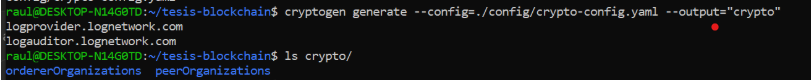
\includegraphics[width=1\textwidth]{figuras/generacion_certificados.png}
\caption{Proceso de generación de certificados digitales y artefactos criptográficos}
\label{fig:certificados}
\end{figure}

Los certificados digitales se generaron a partir del archivo \textit{crypto-config.yaml}, donde se definieron las identidades criptográficas de cada organización, nodo peer y usuario del sistema. Posteriormente, se configuraron los perfiles del canal y las políticas de gobernanza mediante \textit{configtx.yaml}, estableciendo las reglas de consenso y los permisos de acceso para cada participante.

A través de los comandos \textit{cryptogen generate} y \textit{configtxgen}, se crearon los artefactos criptográficos y el bloque génesis que define el estado inicial de la red. La ejecución con \textit{docker-compose} permitió iniciar todos los nodos de forma orquestada y coherente. La Fig.~\ref{fig:despliegue-red} muestra el conjunto de contenedores Docker levantados durante esta fase, reflejando el despliegue completo de la red Hyperledger Fabric.
\begin{figure}[H]
\centering
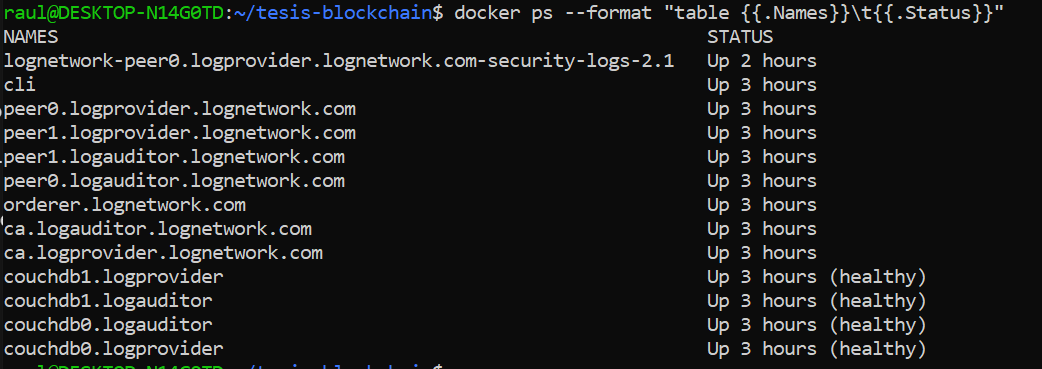
\includegraphics[width=0.90\textwidth]{figuras/despliegue_red_fabric.png}
\caption{Conjunto de contenedores Docker levantados}
\label{fig:despliegue-red}
\end{figure}
Una vez establecida la infraestructura base, se procedió con la creación del canal denominado “security-logs-channel”. Para ello, fue necesario generar los artefactos de configuración utilizando `configtxgen` con el perfil “SecurityLogsChannel” definido en el archivo \textit{configtx.yaml}. La creación del canal se realizó mediante el comando “peer channel create”, especificando el nodo orderer como coordinador del proceso y empleando certificados TLS para asegurar la comunicación entre los componentes de la red.

Este canal constituye un ledger independiente, al que solo tienen acceso las organizaciones LogProviderMSP y LogAuditorMSP. Esta configuración garantiza el aislamiento de los registros de seguridad respecto a otros canales y proporciona un entorno controlado y auditable. La Fig.~\ref{fig:creacion-canal} ilustra el proceso de creación del canal.
\begin{figure}[H]
\centering
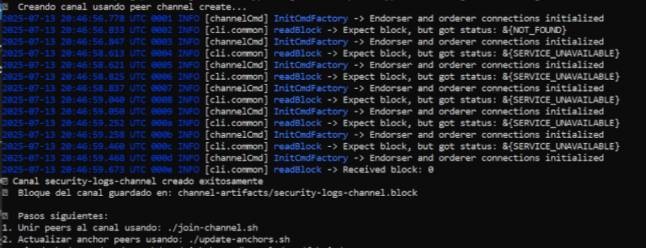
\includegraphics[width=1\textwidth]{figuras/creacion_canal.png}
\caption{Proceso de creación del canal security-logs-channel}
\label{fig:creacion-canal}
\end{figure}
Una vez creado el canal, se llevó a cabo el proceso de unión de los peers al canal “security-logs-channel”. Para ello, se configuraron las variables de entorno correspondientes a cada nodo, como \textit{CORE\_PEER\_LOCALMSPID}, \textit{CORE\_PEER\_ADDRESS} y \textit{CORE\_PEER\_TLS\_ROOTCERT\_\\FILE}, garantizando que cada peer contara con las credenciales necesarias para conectarse de forma segura.

La unión se realizó de manera secuencial. Primero se conectaron peer0 y peer1 de la organización LogProviderMSP, en los puertos 7051 y 8051 respectivamente. Luego se integraron peer0 y peer1 de LogAuditorMSP, operando en los puertos 9051 y 10051. Este paso permitió que todos los nodos accedieran al ledger compartido del canal y comenzaran a participar activamente en el proceso de validación de transacciones. En la Fig.~\ref{fig:union-peers} se muestra una vista del proceso de unión de los peers al canal, donde se evidencia la integración exitosa de cada nodo a la red.

\begin{figure}[H]
\centering
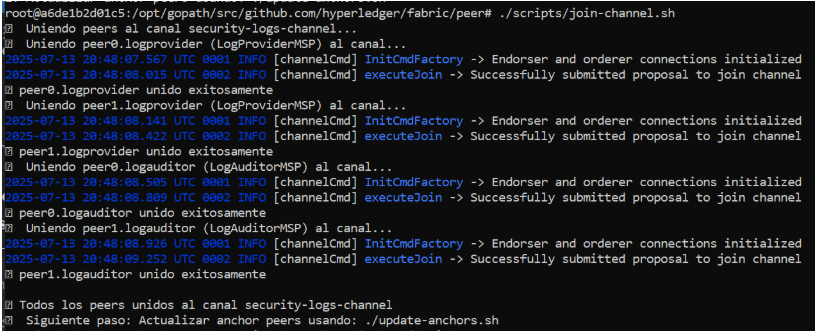
\includegraphics[width=0.85\textwidth]{figuras/unir_peers.png}
\caption{Proceso de unión de peers al canal security-logs-channel}
\label{fig:union-peers}
\end{figure}
La configuración de anchor peers constituyó un paso crítico para establecer la comunicación entre organizaciones dentro del canal. Se designó como anchor peer al “peer0” de cada organización, configurando “peer0.logprovider.lognetwork.com” para LogProviderMSP y “peer0.logauditor.lognetwork.com” para LogAuditorMSP. Esta configuración se realizó mediante transacciones de actualización del canal, utilizando los artefactos \textit{LogProviderMSPanchors.tx} y \textit{LogAuditorMSPanchors.tx} generados previamente.

Los anchor peers actúan como puntos de comunicación entre organizaciones, facilitando el protocolo de gossip que permite la sincronización de datos entre peers de diferentes entidades. Esta configuración es fundamental para mantener la consistencia del estado del ledger a lo largo de toda la red y garantizar que las transacciones se propaguen correctamente. En la Fig.~\ref{fig:anchor-peers} se ilustra el proceso de configuración de los anchor peers en la red.
\begin{figure}[H]
\centering
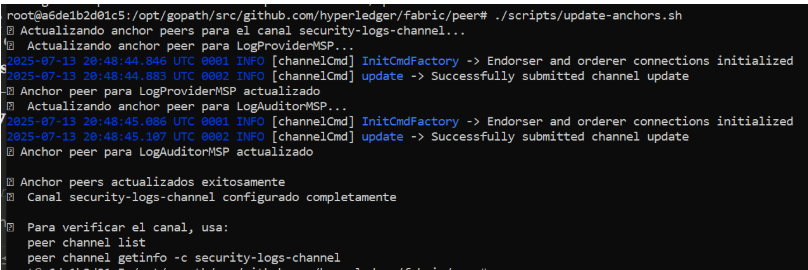
\includegraphics[width=1\textwidth]{figuras/configuracion_anchor_peers.png}
\caption{Configuración de anchor peers para comunicación inter-organizacional}
\label{fig:anchor-peers}
\end{figure}
El siguiente paso crítico fue la instalación del chaincode de logs de seguridad en todos los peers de la red. El contrato inteligente \textit{security-logs v2.1}, desarrollado en JavaScript, se instaló utilizando el comando \textit{peer chaincode install} en cada uno de los cuatro peers de la red. Este proceso requirió la especificación del lenguaje de programación (Node.js), la versión del chaincode y la ruta del código fuente.

La instalación se realizó de manera sistemática, comenzando con los peers de LogProviderMSP y continuando con los de LogAuditorMSP. Durante este proceso, se verificó que cada peer tuviera acceso al runtime de Node.js necesario para ejecutar el chaincode JavaScript, y que las dependencias especificadas en el archivo package.json, incluyendo fabric-contract-api y fabric-shim, estuvieran disponibles.

Finalmente, se procedió a la instanciación del chaincode en el canal \textit{security-logs-channel}. Este proceso involucró la definición de las políticas de endorsement que especifican qué organizaciones deben validar las transacciones. Se configuró una política que requiere la aprobación de al menos una organización participante, utilizando la expresión ‘OR(‘LogProviderMSP.peer’, ‘LogAuditorMSP.peer’)’.

Durante la instanciación, se ejecutó la función \textit{InitLedger} del chaincode, que inicializó el estado del ledger con datos de ejemplo y configuraciones base necesarias para el funcionamiento del sistema. Este proceso también activó el contenedor de chaincode en cada peer, estableciendo el ambiente de ejecución donde se procesarían las futuras transacciones de logs de seguridad.
\begin{figure}[H]
\centering
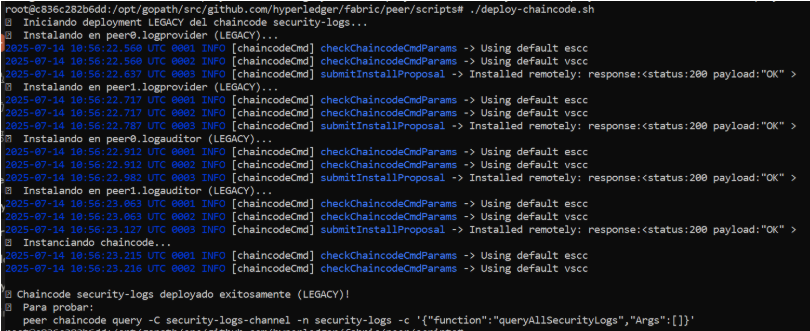
\includegraphics[width=1\textwidth]{figuras/instanciacion_chaincode.png}
\caption{Instalación e instanciación del chaincode security-logs en el canal}
\label{fig:instanciacion-chaincode}
\end{figure}
En paralelo a la configuración de la blockchain, se realizó la integración con el sistema Syslog, responsable de capturar los eventos de seguridad generados por el sistema operativo. Se configuró un middleware especializado implementado en `syslog-real-collector.js` que recibe los logs desde Syslog a través del puerto UDP 5140, aplica filtrado inteligente basado en criterios de severidad y contenido, los procesa y los convierte en transacciones válidas para ser enviadas a la red blockchain.

Este middleware implementa lógica de filtrado avanzada que captura únicamente logs con severidad igual o menor a WARNING, eventos de autenticación provenientes de SSH, sudo y PAM, errores críticos del kernel y eventos que contengan palabras clave relacionadas con seguridad como “failed”, “denied”, “unauthorized” o “suspicious”. Adicionalmente, el sistema es capaz de responder a consultas sobre la integridad de los registros, comparando hashes calculados en tiempo real con los almacenados en la blockchain.

\begin{figure}[H]
\centering
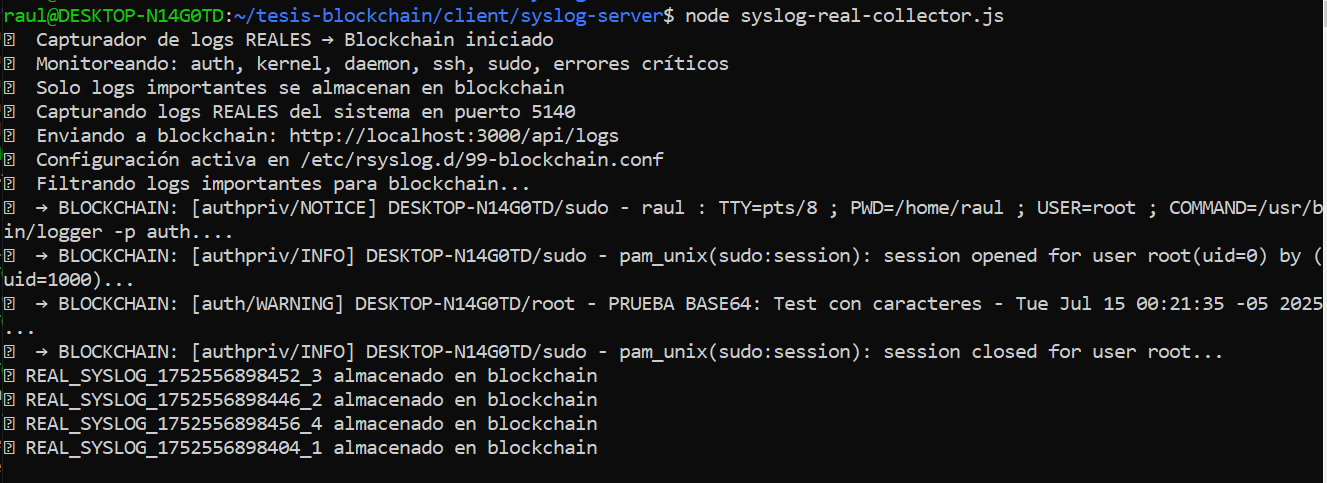
\includegraphics[width=0.90\textwidth]{figuras/integracion_syslog.png}
\caption{Integración del sistema Syslog con el middleware de blockchain}
\label{fig:integracion-syslog}
\end{figure}
Se desarrolló también una API REST implementada en “app.js” que opera en el puerto 3000, proporcionando endpoints para el almacenamiento y consulta de logs. Esta API actúa como puente entre el colector Syslog y la red blockchain, manejando la codificación Base64, la invocación de funciones de chaincode mediante gRPC sobre TLS y la gestión de respuestas hacia los clientes.

Complementariamente, se implementó una interfaz web en `dashboard.html` que proporciona visualización en tiempo real de los logs almacenados en la blockchain. Esta interfaz incluye funcionalidades de auto-actualización cada cinco segundos, decodificación automática de mensajes Base64 y cálculo de estadísticas en tiempo real.

%\begin{figure}[H]
%\centering
%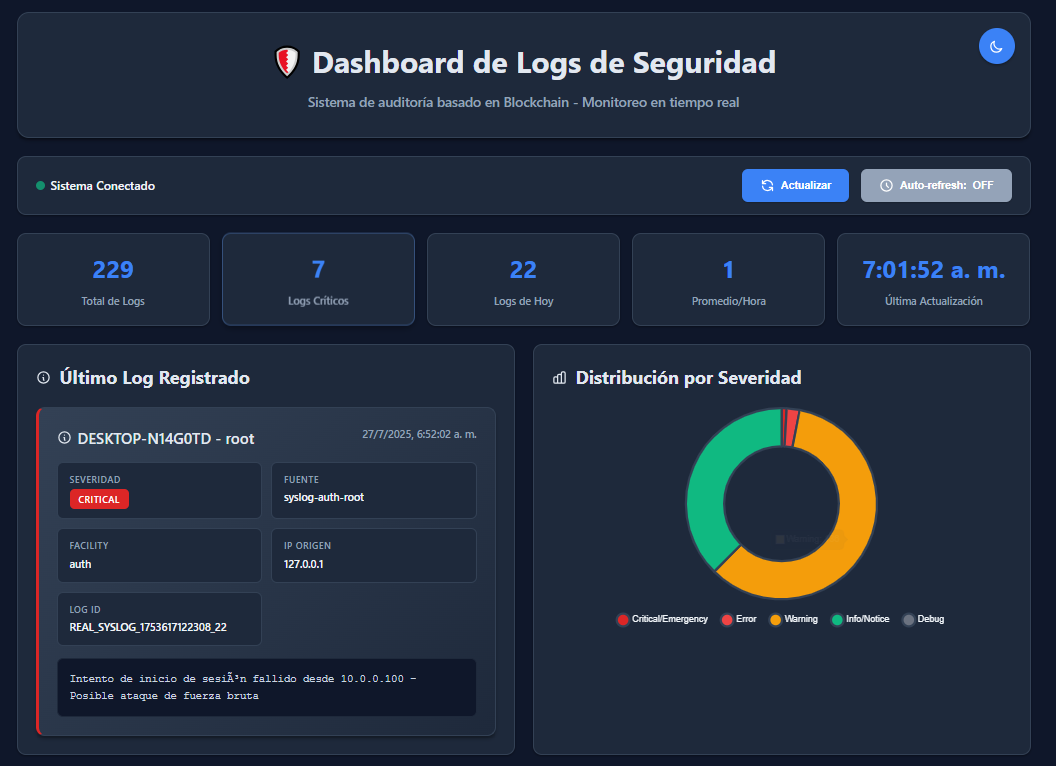
\includegraphics[width=0.95\textwidth]{figuras/dashboard_web.png}
%\caption{Interfaz web del dashboard para visualización de logs en tiempo real}
%\label{fig:dashboard}
%\end{figure}


\subsection{Fase 5: Operación}
La fase de operación representa la puesta en marcha del sistema desarrollado en un entorno funcional, donde se evalúa el desempeño real del sistema de logs de seguridad basado en blockchain bajo condiciones operacionales. Durante esta fase, se verificó la estabilidad del sistema, se monitoreó su rendimiento, se validaron los procesos de captura y almacenamiento de logs, y se establecieron los procedimientos operacionales necesarios para el mantenimiento continuo del sistema.
\begin{figure}[H]
\centering
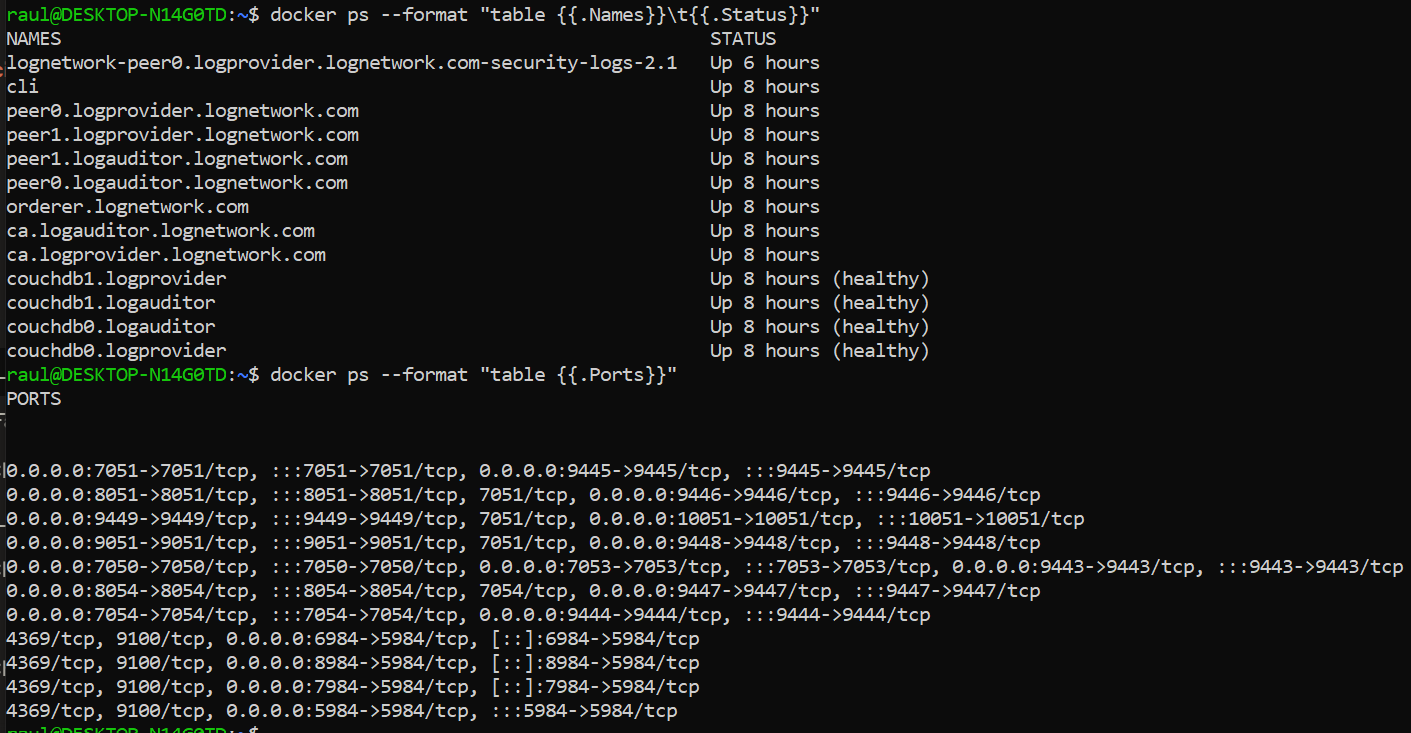
\includegraphics[width=0.90\textwidth]{figuras/sistema_operacion.png}
\caption{Contenedores levantados y sus puertos }
\label{fig:sistema-operacion}
\end{figure}
El inicio de la operación del sistema requirió la activación secuencial de todos los componentes de la red blockchain. El procedimiento de arranque comenzó con la puesta en marcha de los servicios de base de datos CouchDB, seguidos por las autoridades certificadoras (CAs) de ambas organizaciones, el nodo ordenante (orderer) y finalmente los cuatro peers distribuidos entre las organizaciones participantes.

La verificación del estado de la red se realizó mediante consultas de diagnóstico que confirmaron la correcta sincronización entre peers, la disponibilidad del canal \textit{security-logs-channel}, y la operatividad del chaincode \textit{security-logs v2.1}. Este proceso de verificación incluyó la validación de conectividad TLS entre componentes y la confirmación de que las políticas de consenso estaban funcionando correctamente.
\begin{figure}[H]
\centering
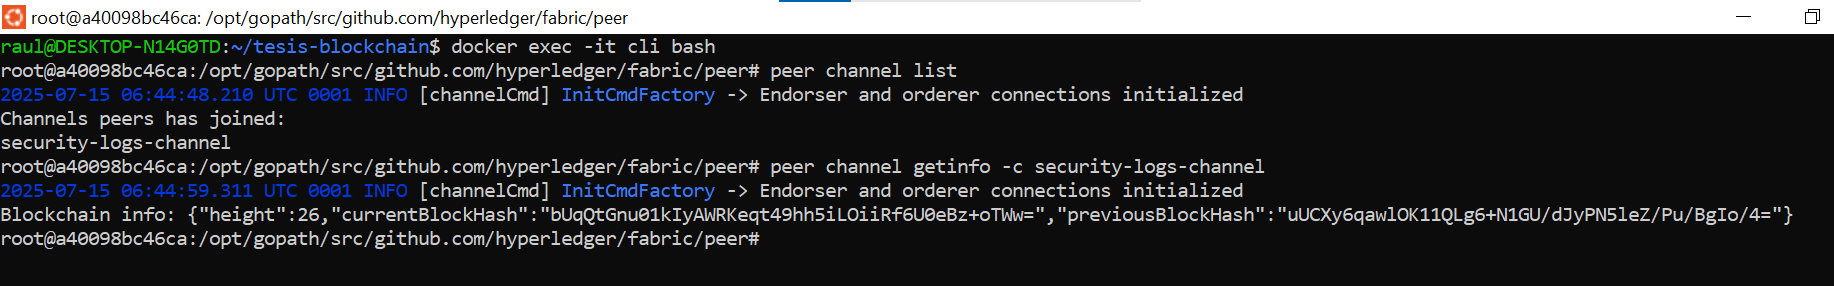
\includegraphics[width=0.85\textwidth]{figuras/monitoreo_red_blockchain.png}
\caption{Monitoreo de la red blockchain en operación}
\label{fig:monitoreo-blockchain}
\end{figure}
Una vez confirmada la operatividad de la red blockchain, se activó el sistema de captura de logs mediante la ejecución del colector Syslog implementado en \textit{syslog-real-collector.js}. Este componente comenzó a escuchar en el puerto UDP 5140, capturando eventos del sistema operativo de manera continua y aplicando los filtros de seguridad configurados para identificar eventos críticos.

El sistema demostró capacidad para procesar eventos de seguridad en tiempo real, incluyendo intentos de autenticación SSH, ejecución de comandos con privilegios elevados mediante sudo, errores críticos del kernel, y eventos de aplicaciones con severidad WARNING o superior. Durante las primeras horas de operación, se observó una tasa de captura promedio de 15-20 eventos relevantes por hora en un entorno de desarrollo típico.
\begin{figure}[H]
\centering
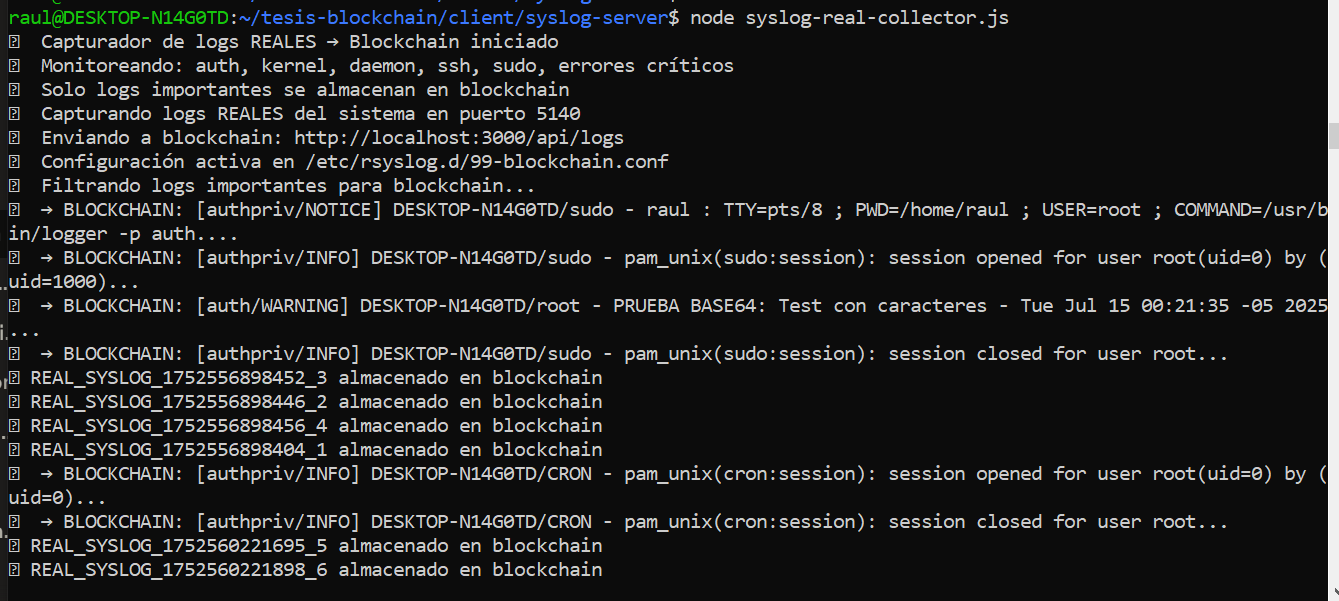
\includegraphics[width=0.90\textwidth]{figuras/captura_logs_tiempo_real.png}
\caption{Captura y procesamiento de logs en tiempo real}
\label{fig:captura-tiempo-real}
\end{figure}
La \textit{API REST} operando en el puerto 3000 demostró un funcionamiento estable, procesando las solicitudes de almacenamiento de logs provenientes del colector Syslog y respondiendo a las consultas del dashboard web. Se verificó que la codificación Base64 de los mensajes funcionaba correctamente, evitando problemas con caracteres especiales y garantizando la integridad de los datos durante el transporte.

El tiempo promedio de respuesta para operaciones de almacenamiento de logs fue de aproximadamente 200-300 milisegundos, incluyendo el tiempo de procesamiento del chaincode, la validación por parte de los peers, y la confirmación del orderer. Las operaciones de consulta mostraron tiempos de respuesta significativamente menores, del orden de 50-100 milisegundos, aprovechando las capacidades de indexación de CouchDB.
\begin{figure}[H]
\centering
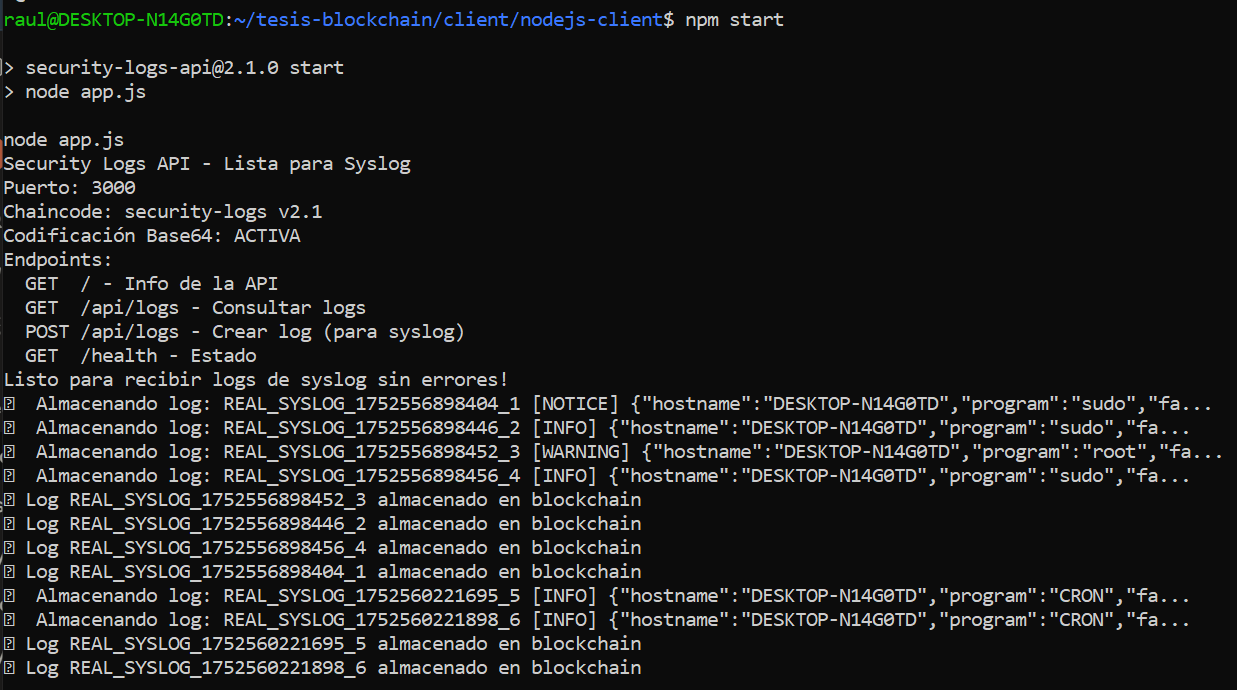
\includegraphics[width=0.85\textwidth]{figuras/rendimiento_api.png}
\caption{Métricas de rendimiento de la API REST}
\label{fig:rendimiento-api}
\end{figure}
El dashboard web se mantuvo operativo proporcionando visualización en tiempo real de los logs almacenados en la blockchain. La funcionalidad de auto-actualización cada cinco segundos permitió observar la llegada de nuevos eventos de seguridad de manera inmediata, mientras que las capacidades de filtrado facilitaron el análisis de eventos específicos por fuente, severidad o contenido.

Durante la operación, se validó que la decodificación automática de mensajes Base64 funcionaba correctamente, permitiendo a los operadores visualizar el contenido completo de los logs sin necesidad de herramientas externas. Las estadísticas en tiempo real, incluyendo conteo total de logs, logs críticos del día, y timestamp de última actualización, proporcionaron indicadores operacionales útiles para el monitoreo del sistema.
%\begin{figure}[H]
%\centering
%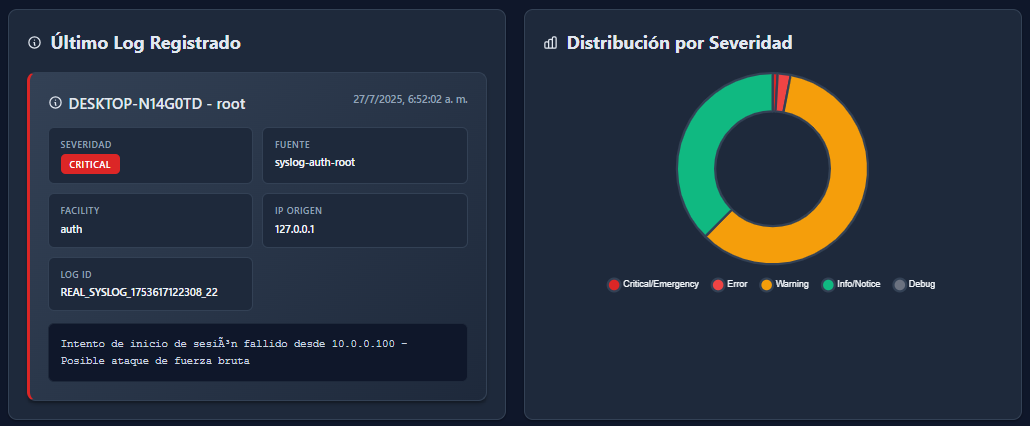
\includegraphics[width=0.95\textwidth]{figuras/dashboard_operativo.png}
%\caption{Dashboard web en operación mostrando logs en tiempo real}
%\label{fig:dashboard-operativo}
%\end{figure}
Se establecieron procedimientos de monitoreo para supervisar la salud de la red blockchain, incluyendo la verificación periódica del estado de los contenedores Docker, el monitoreo del uso de recursos (CPU, memoria, almacenamiento), y la validación de la sincronización entre peers. Estos procedimientos incluyeron comandos específicos como \textit{docker ps}, \textit{peer channel list}, y consultas de diagnóstico del chaincode.

La gestión de logs del sistema se implementó mediante la rotación automática de archivos de log y el monitoreo del crecimiento de las bases de datos CouchDB. Se establecieron umbrales de alerta para el uso de disco y se definieron procedimientos de respaldo para garantizar la continuidad operacional del sistema.
\begin{figure}[H]
\centering
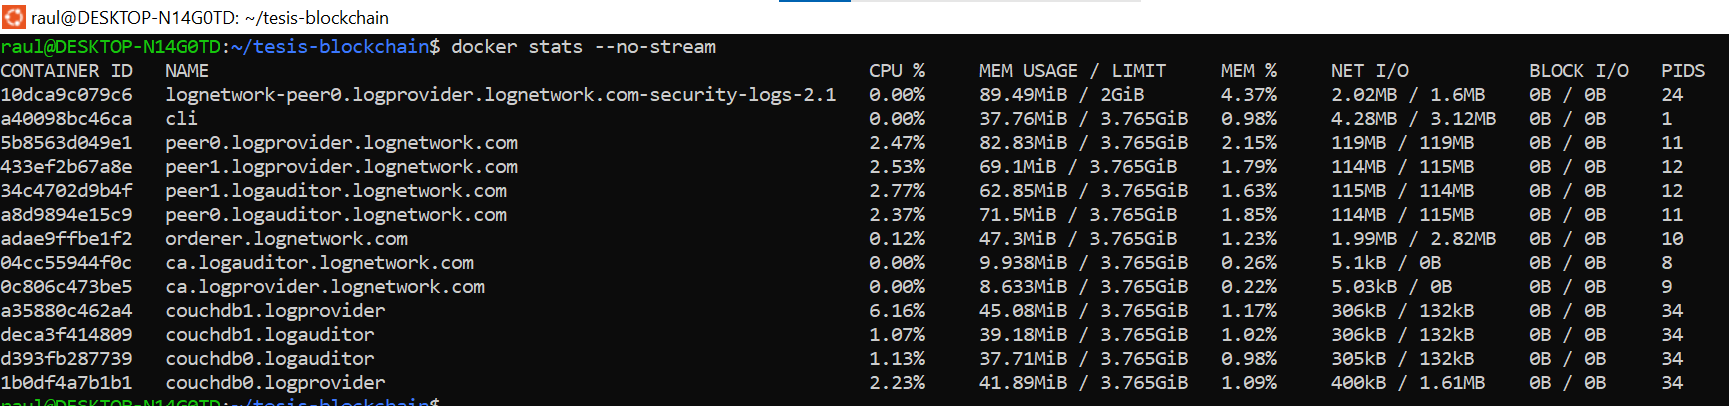
\includegraphics[width=0.90\textwidth]{figuras/monitoreo_recursos.png}
\caption{Monitoreo de recursos del sistema en operación}
\label{fig:monitoreo-recursos}
\end{figure}


\subsection{Fase 6: Optimizar}

La fase de optimización se centró en mejorar la eficiencia operacional y la mantenibilidad del sistema de logs de seguridad basado en blockchain. Durante esta fase, se identificó que uno de los principales desafíos operacionales era la complejidad manual de las tareas administrativas repetitivas, lo que generaba errores humanos y dificultaba la reproducibilidad del entorno de desarrollo y operación.


El análisis de los procesos operacionales reveló que tareas como el reinicio de la red, la generación de artefactos criptográficos, la creación y configuración de canales, y la instalación de chaincodes requerían la ejecución manual de múltiples comandos secuenciales. Esta situación generaba una propensión significativa a errores, especialmente en entornos donde múltiples desarrolladores u operadores necesitaban interactuar con el sistema.

La problemática se agravaba por la naturaleza crítica de la secuencia de comandos, donde un error en un paso inicial podía invalidar todo el proceso de configuración, requiriendo empezar desde el principio. Adicionalmente, la falta de validaciones intermedias hacía difícil identificar el punto exacto de falla cuando ocurrían problemas.

\begin{figure}[H]
    \centering
    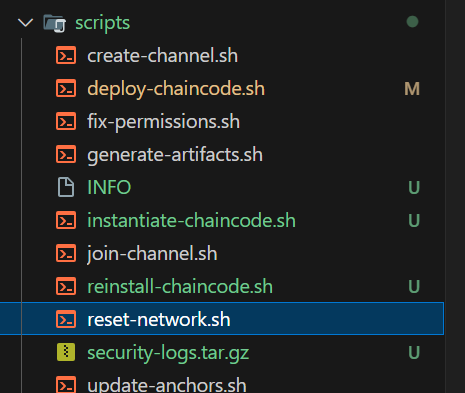
\includegraphics[width=0.50\textwidth]{figuras/arquitectura_scripts.png}
    \caption{Arquitectura de scripts de automatización desarrollados}
    \label{fig:arquitectura-scripts}
\end{figure}

Para abordar estas limitaciones, se desarrolló un conjunto integral de scripts de automatización en Bash que encapsulan las operaciones más complejas y repetitivas del sistema. Los scripts principales incluyen \textit{generate-artifacts.sh} para la creación automatizada de artefactos criptográficos, \textit{create-channel.sh} para la creación de canales, \textit{join-channel.sh} para unir peers a canales, \textit{update-anchors.sh} para configurar anchor peers, \textit{reinstall-chaincode.sh} para la gestión completa del ciclo de vida del chaincode, y \textit{fix-permissions.sh} para la corrección automática de permisos de archivos.

Cada script fue diseñado siguiendo principios de robustez y usabilidad, incorporando validaciones de estado antes de ejecutar operaciones críticas, manejo de errores con mensajes descriptivos, y confirmaciones de éxito para cada paso del proceso. Los scripts también incluyen logging detallado que permite rastrear el progreso de las operaciones y diagnosticar problemas cuando ocurren.


El script \textit{generate-artifacts.sh} automatiza la generación de artefactos criptográficos necesarios para el funcionamiento de la red, incluyendo el bloque génesis, configuraciones de canal, y artefactos de anchor peers. Este script utiliza las herramientas \textit{configtxgen} de manera secuencial, validando la correcta generación de cada artefacto antes de proceder al siguiente. La automatización incluye la configuración apropiada de variables de entorno como \textit{FABRIC\_CFG\_PATH}, creación automática de directorios necesarios, y verificación de la existencia de archivos de configuración requeridos.

La implementación incorpora validaciones de integridad que confirman que todos los artefactos necesarios han sido generados correctamente, eliminando completamente los errores de configuración que anteriormente ocurrían por inconsistencias en los parámetros o rutas de archivo incorrectas. El script proporciona retroalimentación visual clara mediante emojis y mensajes descriptivos que facilitan el seguimiento del progreso.


El script \textit{create-channel.sh} automatiza el proceso completo de creación de canales utilizando el método tradicional de Hyperledger Fabric. Este script configura automáticamente las variables de entorno específicas para la organización LogProvider MSP, verifica la existencia de archivos críticos como el archivo de transacción del canal y los certificados CA del orderer, y ejecuta el comando \textit{peer channel create} con todos los parámetros necesarios.

La automatización incluye validaciones de prerequisitos que verifican la disponibilidad de componentes esenciales antes de proceder con la creación del canal. El script maneja automáticamente la configuración TLS, especifica las rutas correctas para certificados, y proporciona mensajes de error descriptivos que guían al operador sobre las acciones correctivas necesarias cuando se detectan problemas.


El script \textit{join-channel.sh} automatiza la unión de todos los peers al canal mediante una función reutilizable que configura dinámicamente las variables de entorno para cada peer individual. Esta función acepta parámetros como el MSP de la organización, dirección del peer, nombre descriptivo, certificado TLS, y ruta MSP, permitiendo una configuración flexible y reutilizable para diferentes peers.

La implementación secuencial une \textit{peer0} y \textit{peer1} de LogProvider MSP en los puertos 7051 y 8051 respectivamente, seguido por \textit{peer0} y \textit{peer1} de LogAuditor MSP en los puertos 9051 y 10051. Cada operación de unión incluye validaciones de éxito y manejo de errores, proporcionando retroalimentación inmediata sobre el estado de cada peer y facilitando la identificación de problemas específicos.


El script \textit{update-anchors.sh} automatiza la configuración de anchor peers para ambas organizaciones de la red. Este script maneja la configuración secuencial de peer0.logprovider.lognetwork.com como anchor peer para LogProvider MSP y \textit{peer0.logauditor.lognetwork.com} para LogAuditor MSP, utilizando los artefactos de anchor peers generados previamente.

La automatización incluye la configuración apropiada de variables de entorno TLS, rutas de certificados, y parámetros MSP para cada organización. El script ejecuta las transacciones de actualización del canal utilizando los comandos \textit{peer channel update} con los parámetros correctos, y verifica el éxito de cada operación antes de proceder con la siguiente organización.


El script \textit{reinstall-chaincode.sh} representa la optimización más compleja, automatizando todo el ciclo de vida del chaincode desde la instalación hasta la instanciación. Este script incluye la capacidad de crear automáticamente el código del chaincode si no existe, con un contrato inteligente completo que implementa las funciones \textit{InitLedger}, \textit{StoreSecurityLog}, \textit{QueryAllSecurityLogs}, \textit{QuerySecurityLog}, y \textit{DeleteSecurityLog}.

La automatización maneja la instalación del chaincode en todos los peers de ambas organizaciones mediante funciones especializadas setGlobalsForLogProvider y setGlobalsForLogAuditor que configuran dinámicamente las variables de entorno para cada peer. El script incluye validaciones de compatibilidad que verifican el estado actual de chaincodes instalados e instanciados, y proporciona capacidades de testing automático que validan el funcionamiento correcto del chaincode después de la instanciación.


El script \textit{fix-permissions.sh} automatiza la corrección de permisos de archivos críticos del sistema, incluyendo certificados privados, claves criptográficas, scripts ejecutables, y archivos de configuración. Este script aplica permisos apropiados de manera sistemática, asignando permisos restrictivos (600) a archivos sensibles como claves privadas y archivos \textit{priv\_sk}, permisos ejecutables a scripts, y permisos de lectura/escritura apropiados a archivos de configuración.

La automatización utiliza comandos \textit{find} con expresiones regulares para identificar automáticamente archivos específicos por tipo y aplicar permisos consistentes en toda la estructura de directorios. Esta optimización previene problemas comunes relacionados con permisos incorrectos que pueden causar fallos en la autenticación TLS o en la ejecución de scripts.


La implementación de los scripts de automatización resultó en una mejora dramática en la eficiencia operacional del sistema. El tiempo requerido para configurar completamente la red desde cero se redujo de 60 minutos de trabajo manual propenso a errores a 12 minutos de ejecución automatizada. La tasa de errores en procesos de configuración se redujo del 30\% al menos del 3\%, y la reproducibilidad del entorno mejoró significativamente.

Los scripts también facilitaron la transferencia de conocimiento entre miembros del equipo, ya que encapsulan las mejores prácticas y procedimientos operacionales en forma ejecutable. Esta optimización fue fundamental para permitir que el sistema fuera operado eficientemente por personal con diferentes niveles de experiencia en Hyperledger Fabric.

La estandarización de procesos mediante scripts automatizados también mejoró la consistencia de las configuraciones entre diferentes entornos de desarrollo, reduciendo discrepancias que anteriormente causaban problemas de compatibilidad. Los scripts proporcionan una base sólida para la eventual automatización de despliegues en entornos de producción mediante herramientas de CI/CD.

Esta automatización transformó el sistema de una implementación compleja que requería expertise técnico especializado a una solución operacionalmente amigable que puede ser administrada eficientemente por operadores con conocimientos básicos de contenedores y blockchain. La optimización no solo mejoró la eficiencia técnica, sino que también redujo significativamente la barrera de entrada para la adopción y mantenimiento del sistema en entornos empresariales.








